\chapter{D-separation}\label{sec:D-Separation}

% \section{Graphical Models, Directed Acyclic Graph and factorization of joint probability distributions}
Graphical models are an efficient way to describe families of factorized joint distributions of a data set $(x_i)_{i=1,...,n}$ into a \gls{dag}. 

Given such a dataset, we can build a \gls{dag} where each node is indexed by an integer that is higher than the indexes of its \textit{parent} nodes, such that the joint distribution over the dataset factorizes as:

\begin{align}
p(x_1,x_2,...,x_n) = \prod_{i=1}^n p(x_i \vert pa_i)
\end{align}
where $pa_i$ is the set of parent nodes of $x_i$.\\
For example, the following \gls{dag}

% % --- ORIGINAL : WORKS ----------------------
% \begin{center}
% \begin{tikzpicture}[
%     X/.style={circle, draw=black!80, thin, minimum size=5mm}
% ]
% % nodes
% \node[X] (X1) {$x_1$};
% \node[X] (X2) [right= of X1]{$x_2$} edge [<-, thin] (X1); 
% \node[X] (X3) [below= of X1]{$x_3$} edge [<-, thin] (X1);
% \node[X] (X4) [right= of X3]{$x_4$} edge [<-, thin] (X3)
%                                     edge [<-, thin] (X1);
% \node[X] (X5) [right= of X4]{$x_5$} edge [<-, thin] (X4)
%                                     edge [<-, thin] (X2);
% \end{tikzpicture}
% \end{center}
% describes:
% \begin{align}
%     p(x_1,x_2,x_3,x_4,x_5) &= p(x_1)p(x_2\vert x_1)p(x_3\vert x_1)p(x_4 \vert x_1, x_3)p(x_5 \vert x_2, x_4)
% \end{align}

\begin{center}
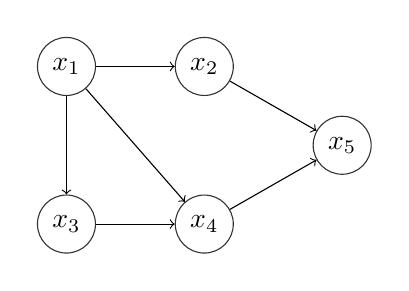
\begin{tikzpicture}[
    X/.style={circle, draw=black!80, thin, minimum size=5mm}
]
% use \matrix to position the nodes
\matrix[row sep=0.25cm, column sep=1cm] {
    % first row
    \node[X] (X1) {$x_1$}; & \node[X] (X2) {$x_2$}; & \\
    & & \node[X] (X5) {$x_5$}; \\
    \node[X] (X3) {$x_3$}; & \node[X] (X4) {$x_4$}; & \\
};
% use \path to draw the edges
\path   (X1) edge[->, thin] (X2)
        (X1) edge[->, thin] (X3)
        (X1) edge[->, thin] (X4)
        (X2) edge[->, thin] (X5)
        (X3) edge[->, thin] (X4)
        (X4) edge[->, thin] (X5);
\end{tikzpicture}
\end{center}
describes:
\begin{align}
    p(x_1,x_2,x_3,x_4,x_5) &= p(x_1)p(x_2\vert x_1)p(x_3\vert x_1)p(x_4 \vert x_1, x_3)p(x_5 \vert x_2, x_4)
\end{align}

% \section{D-separation and conditional independence}

Describing a factorized joint probability distribution by a \gls{dag} allows to determine graphically whether two sets of nodes (ie random variables) are independent, conditioned on a third set of nodes. This allows subsequently to simplify the expressions of the observation models (ie $p(x \vert z)$, and/or the posterior models ($q(z \vert x)$).

\textbf{D-Separation} is the set of rules that determine whether there is conditional independence between two sets given a third one. D-Separation is well described in key books such as \cite{PRML}, \cite{ProbabilisticGraphicalModels} or \cite{ProbabilisticMachineLearning}. We will enunciate here the key concepts, and refer the interested reader to those books.

% \subsection{3-node DAG}

D-Separation is a way to find out graphically conditional (in)dependence relationships between random variables, that would be more difficult to calculate by marginalizing the joint distribution over the conditioning variables. A nice way to demonstrate this, is to review the three examples of 3-node \gls{dag}. 
NB : The observed (ie conditioning) variables are noted with gray background.

% --- EXAMPLE 1 ---------------------------------
\setlength{\columnsep}{1.5cm}
\begin{multicols}{3}[
\textbf{Example 1} : $c$ is said \textit{tail-to-tail} with $a$ and $b$, and \textit{blocks the path between $a$ and $b$}, making them conditionally independent : $a \not\Perp b \cond \varnothing$, $a \Perp b \cond c$
]
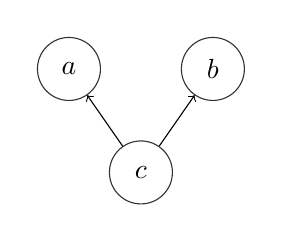
\begin{tikzpicture}[
    UNOBS/.style={circle, draw=black!80, thin, minimum size=8mm},
    OBS/.style={circle, draw=black!80, fill=gray!50, thin, minimum size=8mm}
]
\matrix[row sep=0.5cm, column sep=0.1cm] {
    % first row
    \node[UNOBS] (a) {$a$}; & & \node[UNOBS] (b) {$b$}; & \\
    & \node[UNOBS] (c) {$c$}; & \\
};
\path   (c) edge[->, thin] (b)
        (c) edge[->, thin] (a);
\end{tikzpicture}
% \columnbreak
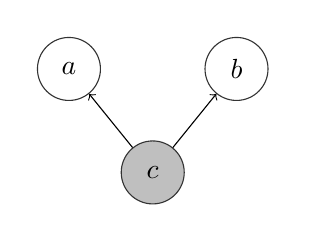
\begin{tikzpicture}[
    UNOBS/.style={circle, draw=black!80, thin, minimum size=8mm},
    OBS/.style={circle, draw=black!80, fill=gray!50, thin, minimum size=8mm}
]
\matrix[row sep=0.5cm, column sep=0.25cm] {
    % first row
    \node[UNOBS] (a) {$a$}; & & \node[UNOBS] (b) {$b$}; & \\
    & \node[OBS] (c) {$c$}; & \\
};
\path   (c) edge[->, thin] (b)
        (c) edge[->, thin] (a);
\end{tikzpicture}
\columnbreak
\begin{align*}
    p(a,b,c) &= p(c)p(a \vert c)p(b \vert c) \\
    p(a,b) &= \sum_c p(c)p(a \vert c)p(b \vert c) \neq p(a)p(b) \\
    &\implies a \not\Perp b \cond \emptyset \\
    p(a,b \vert c) &= p(a \vert c) p(b \vert c) \\
    &\implies a \Perp b \cond c\\
\end{align*}
\end{multicols}


% --- EXAMPLE 2 ---------------------------------
\begin{multicols}{3}[
\textbf{Example 2} : $a,c,b$ form a Markov chain. $c$ is said \textit{head-to-tail} with $a$ and $b$ and, here also, \textit{blocks the path between $a$ and $b$}, making them conditionally independent : $a \notindep b \cond \emptyset$, $a \indep b \vert c$
]
\begin{tikzpicture}[
    UNOBS/.style={circle, draw=black!80, thin, minimum size=8mm},
    OBS/.style={circle, draw=black!80, fill=gray!50, thin, minimum size=8mm}
]
% nodes
\node[UNOBS] (a) {$a$};
\node[UNOBS] (c) [right= of a]{$c$} edge [<-, thin] (a); 
\node[UNOBS] (b) [right= of c]{$b$} edge [<-, thin] (c);
\end{tikzpicture}
% \columnbreak
\vspace{2cm}
\begin{tikzpicture}[
    UNOBS/.style={circle, draw=black!80, thin, minimum size=8mm},
    OBS/.style={circle, draw=black!80, fill=gray!50, thin, minimum size=8mm}
]
% nodes
\node[UNOBS] (a) {$a$};
\node[OBS] (c) [right= of a]{$c$} edge [<-, thin] (a); 
\node[UNOBS] (b) [right= of c]{$b$} edge [<-, thin] (c);
\end{tikzpicture}
\columnbreak
\begin{align*}
    p(a,b,c) &= p(a)p(c \vert a) p(b \vert c) \\
    p(a,b) &\neq p(a)p(b) \implies a \not\Perp b \vert \emptyset \\
    p(a,b \vert c) &= \frac{p(a)p(c \vert a)}{p(c)}p(b \vert c) = p(a \vert c) p(b \vert c) \implies a \Perp b \cond c\\
\end{align*}
\end{multicols}

% --- EXAMPLE 3 ---------------------------------
\setlength{\columnsep}{1.5cm}
\begin{multicols}{3}[
\textbf{Example 3} : $c$ is said \textit{head-to-head} with $a$ and $b$. In this head-to-head configuration, contrary to the two examples above, \textit{the path between $a$ and $b$ is blocked when $c$ is unobserved} : $a \Perp b \cond \emptyset$, $a \not\Perp b \cond c$
]
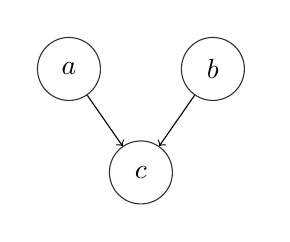
\begin{tikzpicture}[
    UNOBS/.style={circle, draw=black!80, thin, minimum size=8mm},
    OBS/.style={circle, draw=black!80, fill=gray!50, thin, minimum size=8mm}
]
\matrix[row sep=0.5cm, column sep=0.1cm] {
    % first row
    \node[UNOBS] (a) {$a$}; & & \node[UNOBS] (b) {$b$}; & \\
    & \node[UNOBS] (c) {$c$}; & \\
};
\path   (c) edge[<-, thin] (b)
        (c) edge[<-, thin] (a);
\end{tikzpicture}
% \columnbreak
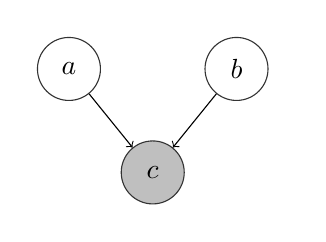
\begin{tikzpicture}[
    UNOBS/.style={circle, draw=black!80, thin, minimum size=8mm},
    OBS/.style={circle, draw=black!80, fill=gray!50, thin, minimum size=8mm}
]
\matrix[row sep=0.5cm, column sep=0.25cm] {
    % first row
    \node[UNOBS] (a) {$a$}; & & \node[UNOBS] (b) {$b$}; & \\
    & \node[OBS] (c) {$c$}; & \\
};
\path   (c) edge[<-, thin] (b)
        (c) edge[<-, thin] (a);
\end{tikzpicture}
\columnbreak
\begin{align*}
    p(a,b,c) &= p(a)p(b)p(c \vert a, b) \\
    p(a,b) &= \sum_c p(a)p(b)p(c \vert a, b) = p(a)p(b) \\ &\implies a \Perp b \cond \emptyset \\
    p(a,b \vert c) &\neq p(a \vert c) p(b \vert c) \\ &\implies a \not\Perp b \cond c\\
\end{align*}
\end{multicols}

% \subsection{General D-Separation theorem}

We can extend the notion to full sets of nodes.

\begin{tcolorbox}[colback=blue!5!white,colframe=black!75!black,title=D-Separation]
    Let $\mathcal{G}$ be a \gls{dag}.
    
    Let $A, B, C$ three disjoint sets of nodes in $\mathcal{G}$ : $A \cap B = A \cap C = B \cap C = \emptyset$. 
    
    $C$ is the set of "conditioning nodes", or "observed variables".

    We aim to determine whether $A \Perp B \cond C$.

    \textbf{Algorithm}
    \begin{enumerate}
        \item \textbf{Evaluate each path between $A$ and $B$}
        
        Evaluate each possible path between any point $a \in A$, and any point $b \in B$. Such a path between $a$ and $b$ is said \textbf {blocked} if it contains one node $n$ such that one of two following conditions is true:
        
            \begin{itemize}
                \item arrows in the path are \textit{head-to-tail} or \textit{tail-to-tail} at node $n$, and $n \in C$ ($n$ is an observed/conditioning node).
                \item arrows in the path are \textit{head-to-head} at node $n$, and $n \notin C$ and none of $n$ descendants is in $C$
            \end{itemize}
            
        \item \textbf{Assess all paths}
            \begin{itemize}
                \item If all paths $(a,b), a \in A, b \in B$ are blocked, then $A$ is said \textbf{D-separated} from $B$ by $C$, and the joint distribution defined by $\mathcal{G}$ verifies $A \Perp B \cond C$.
                \item If there is at least one path $(a,b), a \in A, b \in B$ that is not blocked then $A \not\Perp B \cond C$.
            \end{itemize}
    \end{enumerate}
\end{tcolorbox}